% created for LION#5 
% Time-stamp: "2006-09-12 05:40:55 tpr"
% if all fonts computer modern use -G1
% dvips -Ppdf -G0 <filename>
% http://www.springer.de/comp/lncs/authors.html
\documentclass[10pt]{llncs}

\usepackage[english]{babel}  
\usepackage{latexsym}
\usepackage{amsmath,amssymb}
\usepackage[dvips]{graphicx,psfrag}

\newcommand{\norm}[1]{\lVert#1\rVert}
\renewcommand{\vec}[1]{{\mbox{\boldmath$#1$}}}
\newcommand{\mat}[1]{{\mbox{\boldmath$#1$}}}
\newcommand{\reals}{{\mathbb R}}
\newcommand{\strng}[1]{{\mbox{\tt #1}}}
\newcommand{\inner}[2]{\big<\vec{#1}\cdot\vec{#2}\big>}

\def\argmax{\mathop{\rm argmax}}
\def\argmin{\mathop{\rm argmin}}
\newcommand\bs{\char '134}   
\usepackage{color}

%\newcommand{\mat}[1]{{\mathbf #1}}
\renewcommand{\vec}[1]{{\mathbf #1}}
%\setlength{\textheight}{9.1in} \setlength{\topmargin}{0in} % was 9.3in
%\setlength{\oddsidemargin}{0.18in}\setlength{\evensidemargin}{0.18in}
%\addtolength{\textwidth}{0.2\textwidth}
\hyphenpenalty=800
\hbadness=2500

\title{Supervised Learning Linear Priority Dispatch Rules for Job-Shop Scheduling}

\author{Helga Ingimundardottir \and Thomas Philip Runarsson}
\institute{{School of Engineering and Natural Sciences, University of Iceland}\\
\email{hei2@hi.is} and \email{tpr@hi.is}}
\begin{document}
\maketitle

%\thispagestyle{empty}\pagestyle{empty}
\selectlanguage{english}

\begin{abstract}
This paper introduces a framework in which dispatching rules for job-shop scheduling problems are discovered by analysing the characteristics of optimal solutions. Training data is created via randomly generated job-shop problem instances and their corresponding optimal solution. Linear classification is applied in order to identify good choices from worse ones, at each dispatching time step, in a supervised learning fashion.  The method is purely data-driven, thus less problem specific insights are needed from the human heuristic algorithm designer.  Experimental studies show that the learned linear priority dispatching rules outperforms common single priority dispatching rules, with respect to minimum makespan.
\end{abstract}

\section{Introduction}\label{sec:introduction}

Hand crafting heuristics for NP-hard problems is a time-consuming trial and error process, requiring inductive reasoning or problem specific insights from their human designers. Furthermore, within a problems class, such as job-shop scheduling, it is possible to construct problem instances where one heuristic would outperform another. Given the ad-hoc nature of the heuristic design process there is clearly room for improving the process. Recently a number of attempt have been made to automate the heuristic design process. Here we focus on the job-shop problem. Various learning approaches have been applied to this task such as, reinforcement learning \cite{Dietterich1995}, evolutionary learning \cite{Tay2008}, and supervised learning \cite{Li2005,Malik2007}. The approach taken here is a supervised learning classifier approach.
 
In order to find an optimal (or near optimal) solution for job-shop scheduling problem (JSSP) one could either use exact  methods or heuristics methods. Exact methods guarantee an optimal solution, however, JSSP is NP-hard \cite{Garey1976}. Any exact algorithm generally suffers from the curse of dimensionality, which impedes the application in finding the global optimum in a reasonable amount of time. Heuristics are generally more time efficient but do not necessarily attain the global optimum. A common way of finding a good feasible solution for the JSSP is by applying heuristic dispatching rules, e.g., choosing a task corresponding to longest/shortest operation time;  most/least successors; or ranked positional weight, i.e., sum of operation times of its predecessors. Ties are broken in an arbitrary fashion or by another heuristic rule. Recently it has been shown that combining dispatching rules is promising \cite{Tay2008}, however, there is large number of rules to choose from and so combinations requires expert knowledge or extensive trial-and-error. A summary of over $100$ classical dispatching rules can be found in \cite{Panwalkar1977a}. 
%There is no dominant rule for JSSP, but the most effective have been: most work remaining (MWKR); least work remaining (LWKR); shortest processing time (SPT); and longest processing time (LPT). The classical dispatching rules are continually used in research, but the focus has been on different objectives, e.g. \cite{Chang1996a} minimizes the due-date tightness, or varying the assumptions of the model; \cite{Thiagarajan2005} incorporates different earliness, tardiness and holding costs. In this study we will simply consider minimizing the makespan and ignore all due-date constraints.
% \cite{Drobouchevitch2000,Gao2007} look into solving for bottleneck machines. 
%There has also been some research in reducing JSSP to flow-shop problem, since a lot of jobs in JSSP use the machines in the same order, \cite{Guinet1998a,Ho2007}.

%Instead of using heuristics in creating a JSSP schedule by dispatching one job at a time, one could work with complete feasible schedules and iteratively repairing them for a better result, \cite{Dietterich1995} studied space shuttle payload processing by using reinforcement learning, in particular, TD($\lambda$) learning. They started with a relaxed problem, each job was scheduled as early as its temporal partial order would 	permit. Resource constraints on the machines were initially ignored, called critical path. Then the schedules would be repaired so the resource constraints were satisfied in the minimum amount of iterations.

%\color{red}Start this paper by reviewing automating the heuristic design process... do a lit survey from them at nottingham and special sessions... see the home page of ...\color{black}
%This approach two phased process of construction and improvement is also implemented in timetable scheduling, \cite{Asmuni}. They used a fuzzy approach in considering multiple heuristic ordering in the construction process, and only allowed feasible schedules to be passed to the improvement phase. 

The alternative to hand-crafting heuristics for the JSSP, is to implement an automatic way of learning heuristics using a data driven approach. 
Data can be generated using a known heuristic, such an approach is taken in \cite{Li2005}, where a LPT-heuristic is applied. Then a decision tree is used to create a dispatching rule with similar logic. However, this method cannot outperform the original LPT-heuristic used to guide the search. For instruction scheduling this drawback is confronted in \cite{Malik2007,Russell2009} by using an optimal scheduler, computed off-line. The optimal solutions are used as training data and a decision tree learning algorithm applied as before. Preferring simple to complex models, the resulting dispatching rules gave significantly more optimal schedules than using popular heuristics in that field, and a lower worst-case factor from optimality. A similar approach is taken for timetable scheduling in \cite{Burke2006} using case based reasoning. Training data is guided by the two best heuristics for timetable scheduling. The  authors point out that in order for their framework to be successful, problem features need to be sufficiently explanatory and training data need to be selected carefully so they can suggest the appropriate solution for a specific range of new cases. 

In this work we investigate an approach based on supervised learning on optimal schedules and illustrate its effectiveness by improving upon well known dispatch rules for job-shop scheduling. The approach differs from previous studies, as it uses a simple linear combination of features found using a linear classifier. The method of generating training data is also shown to be critical for the success of the method. In section~\ref{sec:JSSP} priority dispatch rules for the JSSP problem are discussed, followed by a description of the linear classifier in section~\ref{sec:Ordinal}. An experimental study is then presented in section~\ref{sec:Experimental}. The paper concludes with a summary of main findings.


\section{Priority dispatch rules for job-shop scheduling}\label{sec:JSSP}
%In the job shop problem, a set of jobs must be scheduled on a set of machines. Each job consists of a number of operations which are processed on the machines in a predetermined order. The optimal schedule is the one where the time to complete all jobs is minimal (minimum makespan).

The job-shop scheduling task considered here is where $n$ jobs are scheduled on a set of $m$ machines, subject to the constraint that each job must follow a predefined machine order and that a machine can handle at most one job at a time.
% An additional constraint commonly considered are job due-dates, however, due-dates will not be considered here. 
The objective is to schedule the jobs so as to minimize the maximum completion times, also known as the makespan. 

Each job $j$ has an indivisible operation time on machine $a$, $p(j,a)$, which is assumed to be integral, where $j \in\{1,..,n\}$ and $a\in\{ 1,..,m\}$. Starting time of job $j$ on machine $a$ is denoted $x_s(a,j)$ and its completion time is denoted $x_f$ and
\begin{equation}  x_f(a,j)=x_s(a,j)+p(j,a) \end{equation}
Each job has a specified processing order through the machines, it is a permutation vector, $\sigma$, of $\{1,..,m\}$. Representing a job $j$ can be processed on $\sigma(j,a)$ only after it has been completely processed on $\sigma(j,a-1)$, i.e.,
\begin{equation}\label{eq:Permutation}
   x_s( \sigma(j,a),j) \geq x_f(\sigma(j,a-1),j) \quad j\in\{1,..,n\},\; a\in\{2,..,m\}
\end{equation}
The disjunctive condition that each machine can handle at most one job at a time is the following: 
\begin{equation}\label{eq:OneJobPerMac}
   x_s(a,i) \geq x_f(a,j) \quad\textrm{or}\quad x_s(a,j) \geq x_f(a,i)  
\end{equation}
for all $i,j\in\{1,..,n\}$ and $a\in\{1,..,m\}$.  The time in which machine $a$ is idle between jobs $j$ and $j-1$ is called slack time, 
\begin{equation} s(a,j)=x_s(a,j)-x_f(a,j-1). \end{equation}
The makespan is the maximum completion time  
\begin{equation}
  z = \max\{x_f(m,j)\;|\;j=1,..,n\}.
\end{equation}

%\begin{figure}[t!]
%\centering
%\begin{tabular}{ll}
% $n$ & number of jobs in the job-shop\\
% $m$ & number of machines in the job-shop\\
% $p(j,a)$ & processing time for job $j$ on machine $a$,\\ 
% $\sigma(j,a)$ & processing order for job $j$ at time $a$, \\ % $\sigma(j,\cdot)$ is a permutation of $\{1,..,m\}$,\\
% $x_s(a,j)$ & starting time of job $j$ on machine $a$,\\
% $x_f(a,j)$ & completion time of job $j$ on machine $a$,\\
% $s(a,j)$ & the slacktime for machine $a$ between jobs $j$ and $j-1$, \\
%\end{tabular}
%\caption{Notation used in this paper}
%\label{fig:notation}
%\end{figure}

Dispatching rules are of a construction heuristics, where one starts with an empty schedule and adds on one job at a time. When a machine is free the dispatching rule inspects the waiting jobs and selects the job with the highest priority. The priority may depend on which job has the most work remaining (MWKR); least work remaining (LWKR); shortest immediate processing time (SPT); and longest immediate processing time (LPT). These are the most effective dispatching rules. However there are many more available, e.g. randomly selecting an operation with equal possibility (RND); minimum slack time (MST); smallest slack per operation (S/OP); and using the aforementioned dispatching rules with predetermined weights. A survey of more than 100 of such rules was given in 1977 by \cite{Panwalkar1977a}. It has recently been shown that a careful combination of basic dispatching rules can perform significantly better \cite{Jayamohan2004}.

%At each time step, an operation is dispatched which has the highest priority of the ready-list, i.e. the jobs whose previous job from the constraints in \eqref{eq:Permutation} have been assigned. If there is a tie, some other priority measure is used. Generally these priority dispatching rules are static during the scheduling process.


\begin{figure}[b!]
\centering
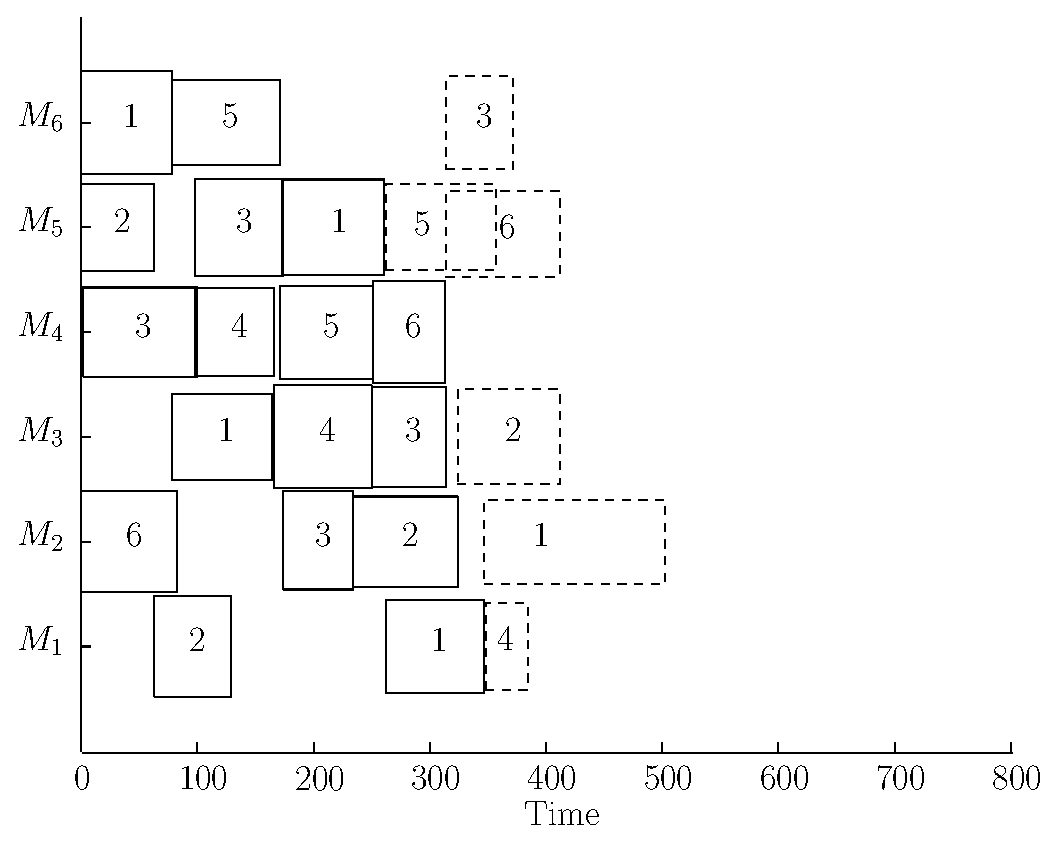
\includegraphics[width=0.8\columnwidth]{figs/dispatch_features.eps}
\caption{A schedule being built, the dashed boxes represent six different possible jobs that could be scheduled next using a dispatch rule.}
\label{fig:dispatch_example}
\end{figure}

In order to apply a dispatching rule a number of features of the schedule being built must be computed. The features of particular interest were obtained from inspecting the aforementioned single priority-based dispatching rules. Some features are directly observed from the partial schedule. The temporal scheduling features applied in this paper for a job $j$ to be dispatched on machine $a$ are: 1) processing time for job $j$ on its next machine $a$; 2) work remaining for job $j$; 3) start-time of job $j$; 4) end-time of $j$; 5) when machine $a$ is next free; 6) current makespan for all jobs; 7) slack time for machine $a$; 8) slack time for all machines; and 9) slack time weighted w.r.t number of number of jobs already dispatched.
Fig.~\ref{fig:dispatch_example} shows an example of a temporal partial schedule for a six job and six machine job-shop problem. The numbers in the boxes represent the job identification $j$. The width of the box illustrates the processing times for a given job for a particular machine $M_i$ (on the vertical axis). The dashed boxes represent the resulting partial schedule for when a particular job is scheduled next. As one can see, there are 17 jobs already scheduled, and 6 potential jobs to be dispatched next. If the job with the shortest processing time were to be scheduled next then job 4 would be dispatched. A dispatch rule may need to perform a one-step look-ahead and observes features of the partial schedule to make a decision, for example by observing the resulting temporal makespan. These resulting observed features are sometimes referred to as an \emph{after-state} or \emph{post-decision state}. Other dispatch rules use features not directly observable from the current partial schedule, for example by assigning jobs with most total processing time remaining. %{\it Other features of importance are the job's starting time $x_s(a,j)$; the time job $j$ will be released $x_f(a,j)$; and the new time machine $a$ will be free again, $x_{\textrm{mac}}(a,j)+p_{\textrm{mac}}(a,j)$; current makespan; sum of slacks; and slacks weighted by number of operations.}

Problem instances are generated stochastically by fixing the number of jobs and machines and sampling a discrete processing time from the uniform distribution $U(R,100)$. The machine order is a random permutation. Two different processing times were explored, namely $U(50,100)$ and $U(1,100)$ for all machines. For each processing time distribution 500 instances were generated for a six job and six machine job-shop problem. Their optimal solution were then found using the GNU linear programming kit \cite{GLPK}. 
The optimal solutions are used to determine which job should be dispatched in order to create an optimal schedule and which ones are not. When a job is dispatched the features of the partial schedule change. The aim of the linear learning algorithm, discussed in the following section, is to determine which features are better than others. That is, features created when a job is scheduled in order to build the known optimal solution as opposed to features generated by dispatching jobs that will result in a sub-optimal schedule.



\section{Logistic Regression}\label{sec:Ordinal}

The preference learning task of linear classification presented here is based on the work presented in \cite{liblinear,newtontrustregion}. The modification relates to how the point pairs are selected and the fact that a $L2$-regularized logistic regression is used. 

Let $\vec{\phi}^{(o)}\in\mathbb{R}^d$ denote the post-decision state when the job dispatched corresponds to an optimal schedule being built. All post-decisions states corresponding to suboptimal dispatches are denoted by $\vec{\phi}^{(s)}\in\mathbb{R}^d$. One could label which feature sets were considered optimal, $\vec{z}_o=\vec{\phi}^{(o)}-\vec{\phi}^{(s)}$, and suboptimal, $\vec{z}_s=\vec{\phi}^{(s)}-\vec{\phi}^{(o)}$ by $y_o=+1$ and $y_s=-1$ respectively. 
Note, a negative example is only created as long as the job dispatched actually changed the resulting makespan, since there can exist situations in which more than one choice can be considered optimal.

The preference learning problem is specified by a set of preference pairs:
\begin{equation}
S = \left\{\left\{\vec{\phi}^{(o)}-\vec{\phi}^{(s)}_j,+1)\right\}_{k=1}^{\ell},\left\{\vec{\phi}^{(s)}_j-\vec{\phi}^{(o)},-1)\right\}_{k=1}^{\ell}
\;|\;\forall j\in J^{(k)}
\right\}\subset \Phi\times Y
\end{equation}
where $\Phi\subset \mathbb{R}^d$ is the training set of $d$ features, $Y=\{-1,+1\}$ is the outcome space, $\ell=n\times m$ is the total number of dispatches and $j\in J^{(k)}$ are the possible suboptimal dispatches at dispatch $(k)$. 
In this study, there are $d=9$ features, and the training set is created from known optimal sequences of dispatch.

Now consider the model space $h\in\mathcal{H}$ of mappings from points to preferences. Each such function $h$ induces an ordering $\succ$ on the points by the following rule:
\begin{equation}
 \vec{\phi}^{(o)}\succ\vec{\phi}^{(s)} \quad \Leftrightarrow \quad h(\vec{\phi}^{(o)})>h(\vec{\phi}^{(s)})
\end{equation}
where the symbol $\succ$ denotes ``is preferrred to''. 
The function used to induce the preference is defined by a linear function in the feature space:
\begin{equation}
 h(\vec{\phi})=\sum_{i=1}^d w_i\phi_i.
\end{equation}

Let $\vec{z}$ denote either $\vec{\phi}^{(o)}-\vec{\phi}^{(s)}$ with $y=+1$ or $\vec{\phi}^{(s)}-\vec{\phi}^{(o)}$ with $y=-1$ (positive or negative example respectively).
Logistic regression learns the optimal parameters $\vec{w}\in\mathbb{R}^d$ determined by solving the following task:
\begin{equation}\label{eq:margin}
\min_{\vec{w}}\quad \tfrac{1}{2}\inner{w}{w} + C \sum_{i=1}^l \log\left(1 + e^{-y_i \inner{w}{z_i}}\right) 
\end{equation}
where $C > 0$ is a penalty parameter, and the negative log-likelihood is due to the fact the given data points $\vec{z}$ and weights $\vec{w}$ are assumed to follow the probability model:
\begin{equation}\label{eq:prob}
 P(y=\pm1|\vec{z},\vec{w})=\frac{1}{1+e^{-y\inner{w}{z}}}.
\end{equation}
The logistic regression defined in \eqref{eq:margin} is solved iteratively, in particular using Trust Region Newton method \cite{newtontrustregion}, which generates a sequence $\{\vec{w^{(k)}}\}_{k=1}^\infty$ converging to the optimal solution $\vec{w}^*$ of \eqref{eq:margin}.

The regulation parameter $C$ in \eqref{eq:margin}, controls the balance between model complexity and training errors, and must be chosen appropriately. It is also important to scale the features $\vec{\phi}$ first. A standard method of doing so is by scaling the training set such that all points are in some range, typically $[-1,1]$. That is, scaled $\tilde{\vec{\phi}}$ is
\begin{equation}\label{eq:scale}
\tilde \phi_i = 2 (\phi_i - \underline{\phi}_i) / (\overline{\phi}_i - \underline{\phi}_i) - 1 ~~~ i = 1,\ldots,d
\end{equation}
where $\underline{\phi}_i$, $\overline{\phi}_i$ are the maximum and minimum $i$-th component of all the feature variables in set $\Phi$. Scaling makes the features less sensitive to process times.

Logistic regression makes optimal decisions regarding optimal dispatches and at the same time efficiently estimates a posteriori probabilities. The optimal $\vec{w}^*$ obtained from the training set, can be used on any new data point, $\vec{\phi}$, and their inner product is proportional to probability estimate \eqref{eq:prob}. Hence, for each feasible job $j$ that may be dispatched, $\vec{\phi}_j$ denotes the corresponding post-decision state. The job chosen to be dispatched, $j^*$, is the one corresponding to the highest preference estimate, i.e 
\begin{equation}\label{eq:lin}
j^*=\argmax_{j} h(\vec{\phi}_j)
\end{equation}
where $h(\cdot)$ is the linear classification model ($lin$) obtained by the training data. 

\section{Experimental Study}\label{sec:Experimental}

In the experimental study we investigate the performance of the linear dispatch\-ing rules trained on problem instance generated using production times according to distributions $U(1,100)$ and $U(50,100)$. The resulting linear models is referred to as $lin_{U(1,100)}$ and $lin_{U(50,100)}$, respectively. These rules are compared with the single priority dispatching rules mentioned previously. The goal is to minimize the makespan, here the optimum makespan is denoted $\mu_{\text{opt}}$, and the makespan obtained from a dispatching rule by $\mu_{\text{DR}}$. Since the optimal makespan varies between problem instances the following performance measure is used:
\begin{equation}\label{eq:ratio}\rho=\frac{\mu_{\text{DR}}}{\mu_{\text{opt}}}\end{equation}
which is always greater or equal to 1.

There were 500 problem instances generated using six machines and six jobs, for both $U(1,100)$ and $U(50,100)$ processing times distributions. %Training data generated from these instances is then split up into 200 for training, 100 for validation (used to optimize the parameters of the learning algorithm) and 200 for testing. 
Throughout the experimental study, a Kolmogorov-Smirnov goodness-of-fit hypothesis test with a significance level 0.05 is used to check if there is a statistical difference between the models in question.

\subsection{Data generation}\label{sec:datagen}

An optimal sequence of job dispatches is known for each problem instance. The sequence indicates in which order the jobs should be dispatched. 
A job is placed at the earliest available time slot for its next machine, whilst still fulfilling constraints \eqref{eq:Permutation} and \eqref{eq:OneJobPerMac}. 
%that each machine can handle at most one job at each time, and jobs need to have finished their previous machines according to its machine order. 
Unfinished jobs are dispatched one at a time according to the optimal sequence. After each dispatch the schedule's current features are updated based on the half-finished schedule. This sequence of job assignments is by no means unique. Take for instance Fig.~\ref{fig:dispatch_example}, let's say job \#1 would be dispatched next, and in the next iteration job \#2. Now this sequence would yield the same schedule as if job \#2 would have been dispatched first and then job \#1 in the next iteration. In this particular instance one could not infer that choosing job \#1 is optimal and \#2 is suboptimal (or vice versa) since they can both yield the same optimal solution, however the state of the schedule has changed and thus its features. Care must be taken in this case that neither resulting features are labeled as undesirable. Only the resulting features from a dispatch resulting in a suboptimal solution should be labeled undesirable. This is the approach taken here. Nevertheless, there may still be a chance that having dispatched a job resulting in a different makespan would have resulted in the same makespan if another optimal scheduling path were to have been chosen. That is, there are multiple optimal solutions to the same problem instance. We will ignore this for the current study, but note that our data may be slightly corrupted for this reason. In conclusion, at each time step a number of feature pair are created, they consist of the features resulting from optimal dispatch versus features resulting from suboptimal dispatches.
%The optimal choice is compared with other possible suboptimal choices, and if the makespan would worsen, a optimal/suboptimal pair according to \eqref{eq:pair} is created, however if the makespan would be unaltered the pair is omitted since they give the same optimal makespan. 

When building a complete schedule $n\times m$ dispatches must be made sequentially. At each dispatch iteration a number of data pairs are created which can then be multiplied by the number of problem instance created. We deliberately create a separate data set for each dispatch iterations, as our initial feeling is that dispatch rules used in the beginning of the schedule building process may not necessarily be the same as in the middle or end of the schedule. As a result we will have $n\times m$ linear scheduling rules for solving a $n \times m$ JSSP.

%Due to the non-uniqueness of the sequence representation, incorrect labelling of the training data for that segment can occur. 
%This is solved by comparing the optimal choice with other possible suboptimal choices, by checking if the makespan would change if the current optimal step is changed in the optimal sequence to one of the other possible choices, and substituting the next occurrence with the suboptimal choice with the optimal one. 

\subsection{Training size and accuracy}\label{sec:Expr:Train}
%There were 500 instances of optimal schedules created for each data distribution, which needed to be divided into a training and test set. 

%Training data generated from these instances is then split up into 200 for training, 100 for validation (used to optimize the parameters of the learning algorithm) and 200 for testing. 
Of the 500 schedule instances, 20\% were devoted solely to validation, in order to optimize the parameters of the learning algorithm. Fig.~\ref{fig:train_size} shows the ratio from optimum makespan, $\rho$ in \eqref{eq:ratio}, of the validation set as a function of training size for both processing time distributions considered. As one might expect, a larger training set yields a better result. However, a training size of only 200 is deemed sufficient for both distributions, and will be used here on after, yielding the remaining unused 200 instances as its test set. The training accuracy reported by the $lin$-model during training with respect to choosing the optimal job at each time step is depicted in Fig.~\ref{fig:train_acc} for both data distribution considered. The models obtained from using the training set corresponding to  $U(1,100)$ and $U(50,100)$ data distributions are referred to as $lin_{U(1,100)}$ and $lin_{U(50,100)}$, respectively. 
%It is noted that there is no statistical difference\footnote{Kolmogorov-Smirnov goodness-of-fit hypothesis test with a significance level $0.05$.} between the training accuracy between the two models. 
The training accuracy, that is the ability to dispatch jobs according to an optimal solution, increases as more jobs are dispatched. This seems reasonable since the features initially have little meaning and hence are contradictory. It becomes easier to predict good dispatches towards the end of the schedule. This illustrates the care needed in selecting training data for learning scheduling rules. %Which is to be expected, since due to the predetermined ordering in which the jobs can be schedules leaves less and less options in order to choose from.

\begin{figure}[t!]
\centering
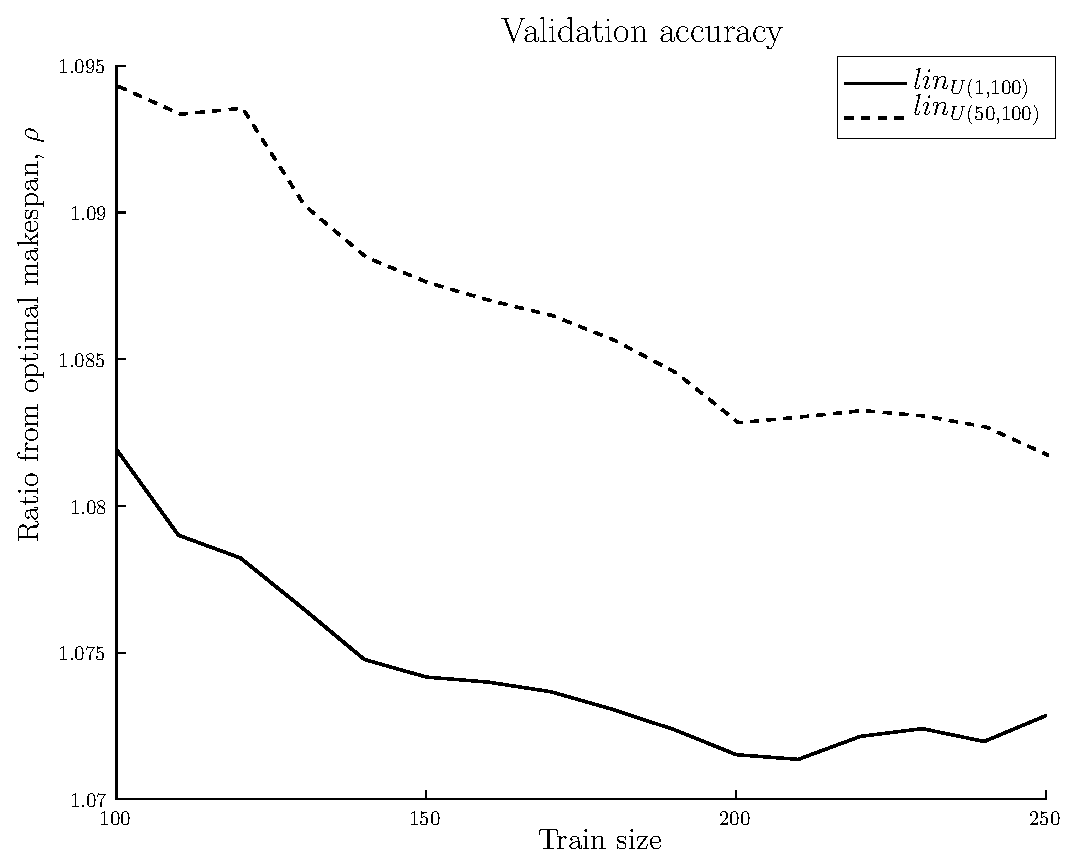
\includegraphics[width=.7\columnwidth]{figs/fig1_trainsize.eps}
\caption{Ratio from optimum makespan, $\rho$, for the validation set as a function of size of training set. Solid line represents model $lin_{U(1,100)}$ and dashed line represents model $lin_{U(50,100)}$.}\label{fig:train_size}
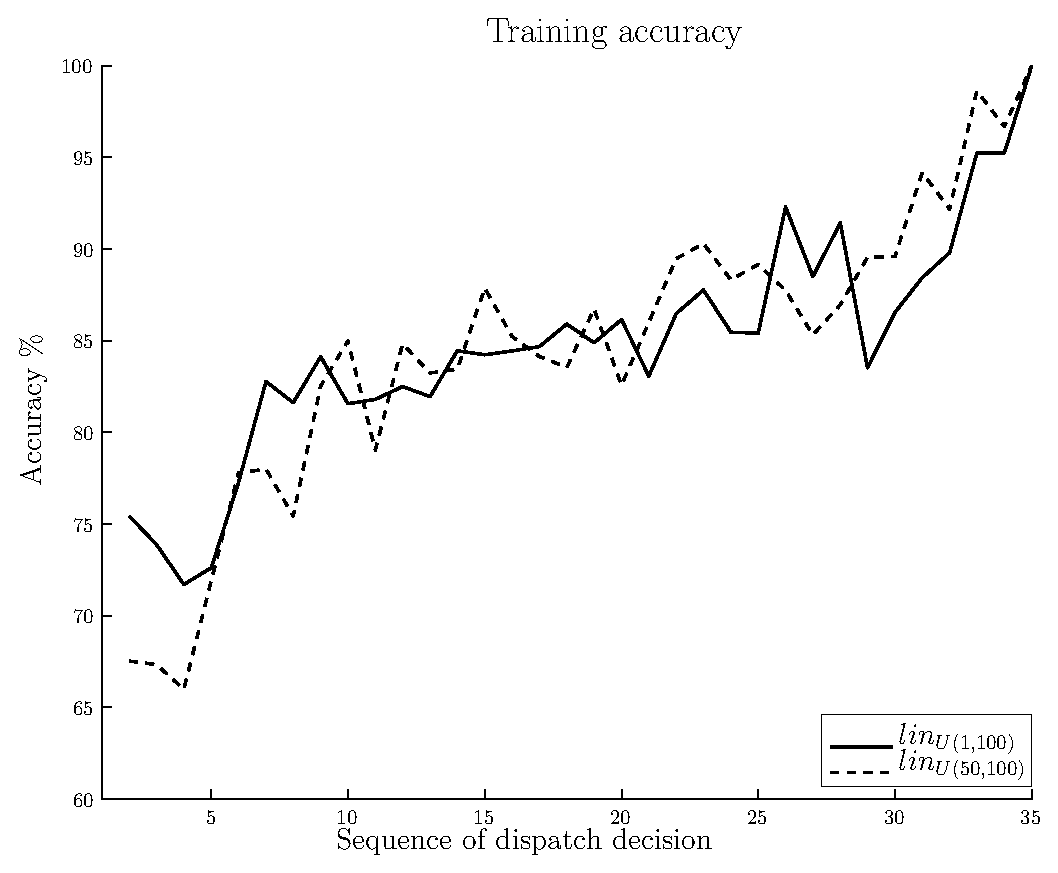
\includegraphics[width=.7\columnwidth]{figs/fig2_trainacc.eps}
\caption{Training accuracy as a function of sequence of dispatching decisions. Solid line represents model $lin_{U(1,100)}$ and dashed line represents data distributions $lin_{U(50,100)}$.}\label{fig:train_acc}
\end{figure}


\subsection{Comparison with single priority dispatching rules}
The performance of the two learned linear priority dispatch rules, ($lin_{U(1,100)}$, $lin_{U(50,100)}$), are now compared with the three most common single priority-based dispatching rules from the literature, which dispatch according to: operation with shortest processing time ($SPT$), most work remaining ($MWRM$), and least work remaining ($LWRM$). 
%Three single priority-based dispatching rules from the literature were compared with our two learned linear priority dispatch rule. 
Their ratio from optimum, \eqref{eq:ratio}, is depicted in Fig.~\ref{fig:densities}, and corresponding statistical findings are presented in Table~\ref{tbl:stats}. Clearly model $lin_{U(R,100)}$ outperforms all conventional single priority-based dispatching rules, but of them $MWRM$ is the most successful. It is interesting to note that for both data distributions, the worst-case scenario (right tail of the distributions) for model $lin_{U(R,100)}$ is noticeably better than the mean obtained using dispatching rules $SPT$ and $LWRM$, so the choice of an appropriate single dispatching rule is of paramount importance.

\begin{figure}[h!]
\centering
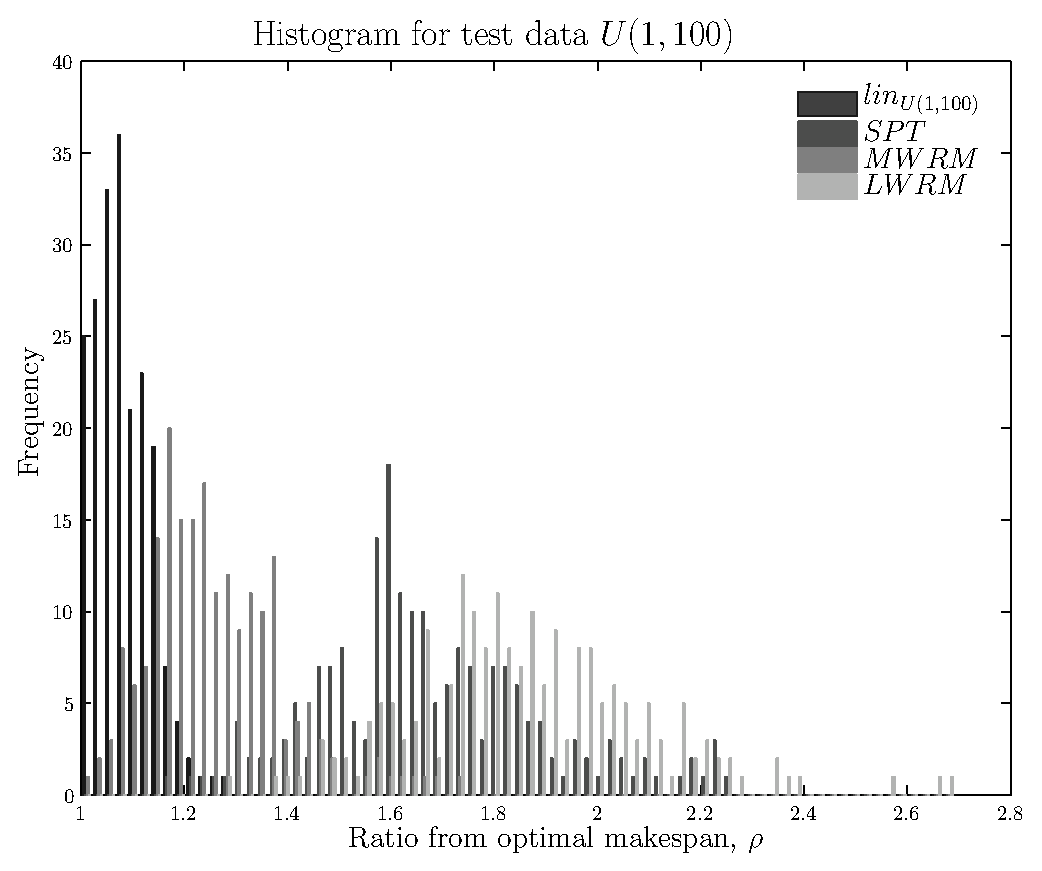
\includegraphics[width=0.82\columnwidth]{figs/fig3_hist_0_100.eps}
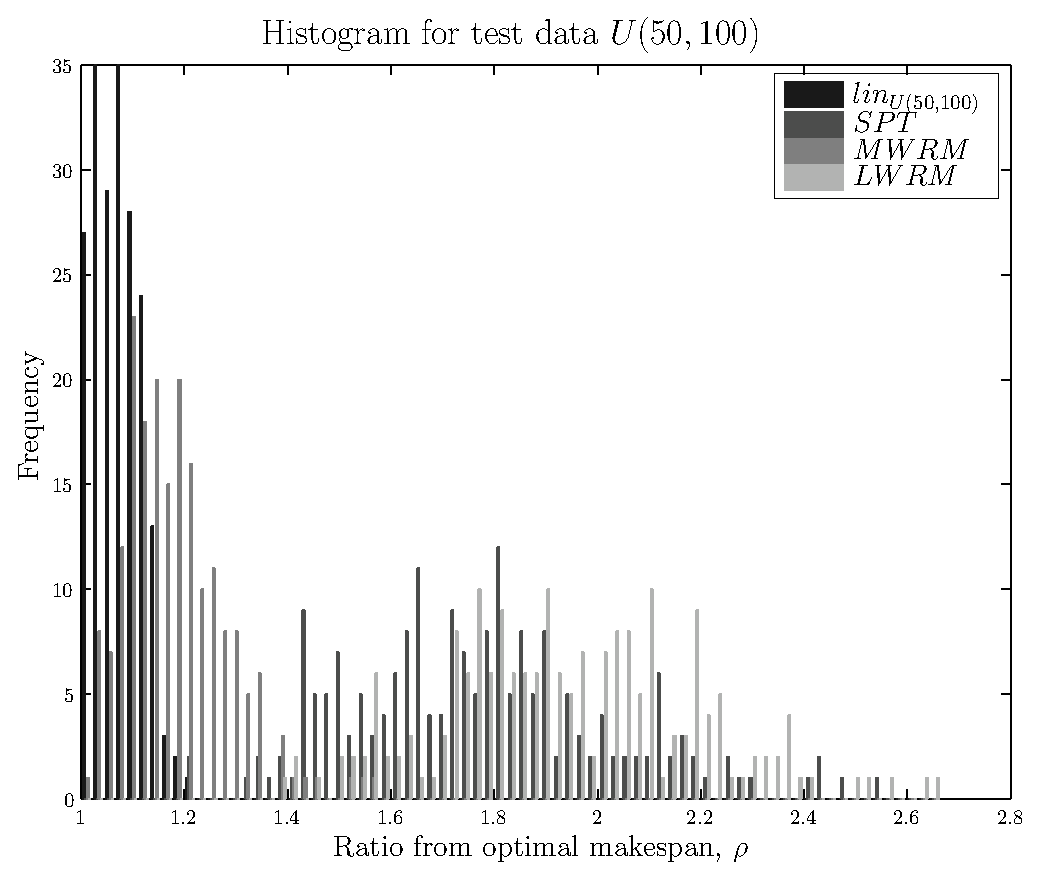
\includegraphics[width=0.82\columnwidth]{figs/fig3_hist_50_100.eps}
\caption{Histogram of ratio $\rho$ for the dispatching rules $lin_{U(R,100)}$, $SPT$, $MWRM$ and $LWRM$ for models $lin_{U(1,100)}$ (top) and $lin_{U(50,100)}$ (bottom).}
\label{fig:densities}
\end{figure}


\begin{table}[t!]
 {\footnotesize
 \begin{center}
  \begin{tabular}{|p{1.5cm}|ccccc|}
   \hline\hline
   $U(1,100)$ & mean& std    & med    & min    & max   \\ \hline
   $lin_{U(1,100)}$ & 1.0842 & 0.0536 & 1.0785 & 1.0000 & 1.2722\\
   $SPT$     & 1.6707 & 0.2160 & 1.6365 & 1.1654 & 2.2500\\
   $MWRM$    & 1.2595 & 0.1307 & 1.2350 & 1.0000 & 1.7288\\
   $LWRM$    & 1.8589 & 0.2292 & 1.8368 & 1.2907 & 2.6906\\  
   \hline\hline
  \end{tabular}
  \begin{tabular}{|p{1.5cm}|ccccc|}
   \hline\hline
   $U(50,100)$ & mean   & std    & med    & min    & max    \\ \hline
   $lin_{U(50,100)}$    & 1.0724 & 0.0446 & 1.0713 & 1.0000 & 1.2159 \\
   $SPT$         & 1.7689 & 0.2514 & 1.7526 & 1.2047 & 2.5367 \\ 
   $MWRM$        & 1.1835 & 0.0994 & 1.1699 & 1.0217 & 1.5561 \\
   $LWRM$        & 1.9422 & 0.2465 & 1.9210 & 1.3916 & 2.6642 \\ 
   \hline\hline
  \end{tabular}
 \end{center}}
 \caption{Mean value, standard deviation, median value, minimum and maximum values of the ratio from optimum makespan, $\rho$, using the test sets $U(1,100)$ (top) and $U(50,100)$ (bottom) .}
 \label{tbl:stats}
\end{table}


\subsection{Robustness towards data distributions}\label{sec:Expr:Robust}
%As can be seen in subsection~\ref{sec:Expr:Train}, the data distributions show a similar behavior in training accuracy with respect to choosing the next optimal step in the sequence of dispatching decision (Figure~\ref{fig:train_acc}). 
All features are scaled according to \eqref{eq:scale}, which may enable the dispatch rules to be less sensitive to the different processing time distributions. 
To examine this the dispatch rules $lin_{U(1,100)}$ and $lin_{U(50,100)}$ are tested on both $U(1,100)$ and $U(50,100)$ test sets. The statistics for $\rho$ are presented in Table~\ref{tbl:diffdatadistr}. 
There is no statistical difference between series \#1 and \#4, implying that when the dispatch rules are tested on their corresponding test set, they perform equally well. It is also noted that there is no statistical difference between series \#2 and \#4, implying that rule $lin_{U(50,100)}$ performed equally well on both test sets in question. However, when observing at the test sets, then in both cases there is a statistical difference between applying model $lin_{U(1,100)}$ or $lin_{U(50,100)}$, where the latter yielded a better results. This implies that the rules are actually not robust towards different data distributions in some cases. This is as one may have expected.

%\begin{figure}[b!]
%\centering
%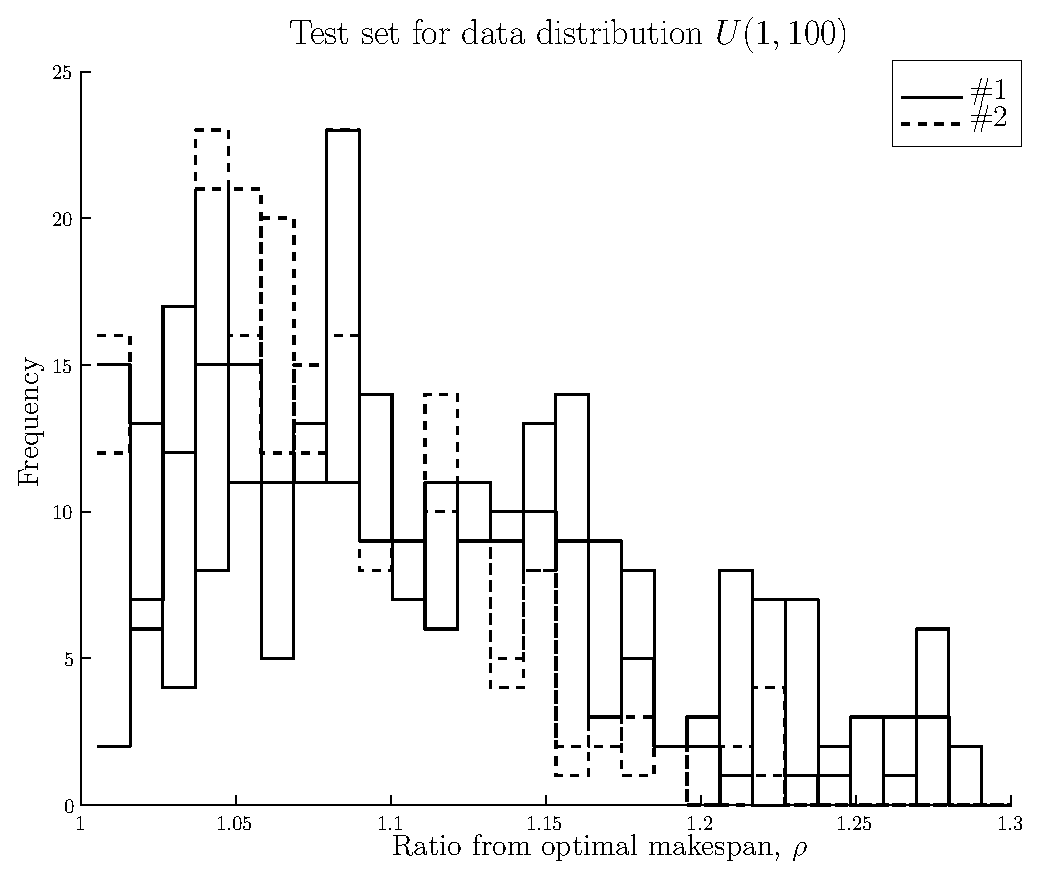
\includegraphics[width=0.49\columnwidth]{figs/fig4_hist0_100.eps}
%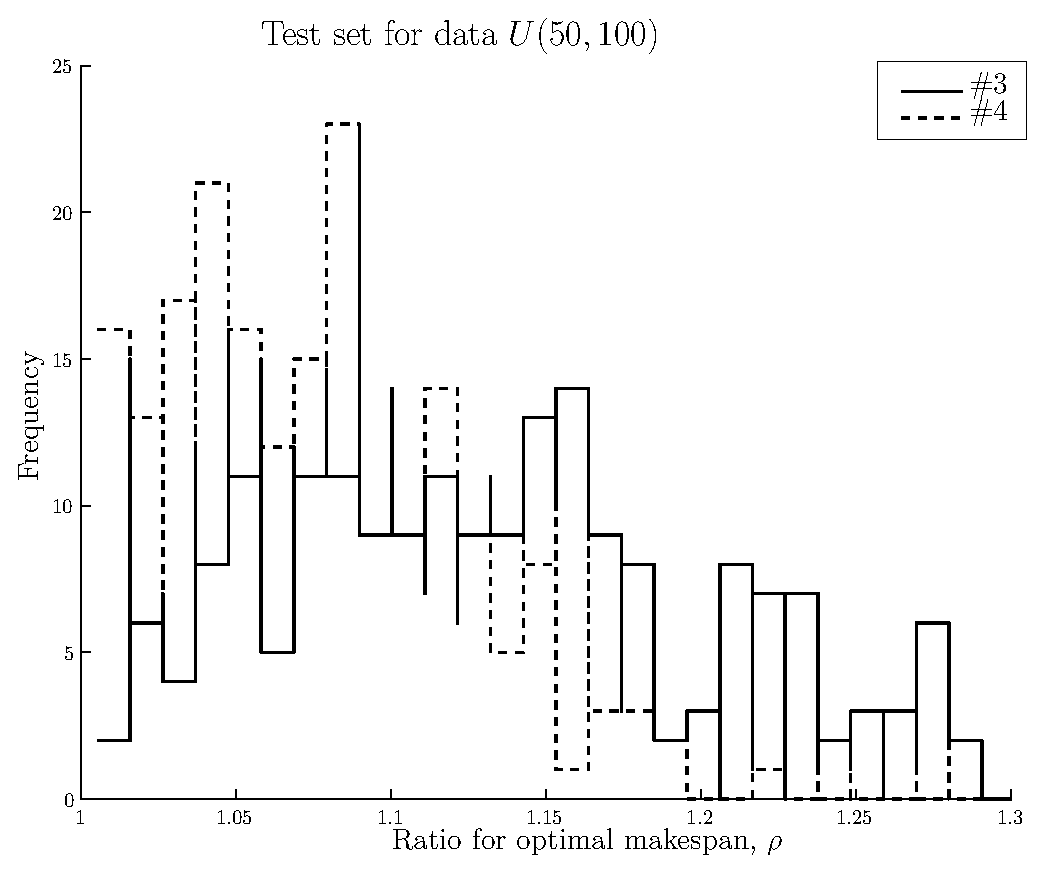
\includegraphics[width=0.49\columnwidth]{figs/fig4_hist50_100.eps}
%\caption{Histogram of deviation from optimum makespan for the dispatching rules using model trained on either $U(1,100)$ or $U(50,100)$ and tested on both $U(1,100)$ (left) and $U(50,100)$ (right).}
%\label{fig:diffdatadistrdensities}
%\end{figure}

\begin{table}[t!]
 {\footnotesize
 \begin{center}
  \begin{tabular}{|c|l|l|ccccc|}
   \hline\hline
   & model & test set & mean & std    & med    & min    & max   \\ \hline
\#1 & $lin_{U(1,100)}$ & $U(1,100)$ & 1.0844 & 0.0535 & 1.0786 & 1.0000 & 1.2722  \\
\#2 & $lin_{U(50,100)}$ & $U(1,100)$ & 1.0709 & 0.0497&1.0626 & 1.0000 & 1.2503  \\
\#3 & $lin_{U(1,100)}$ & $U(50,100)$ & 1.1429 & 0.1115&1.1158 & 1.0000 & 1.5963  \\
\#4 & $lin_{U(50,100)}$ & $U(50,100)$ & 1.0724 & 0.0446&1.0713 & 1.0000 & 1.2159  \\
%#4 and #2 are the same distribution
%#4 and #1 are the same distribution
   \hline\hline
  \end{tabular}
 \end{center}}
 \caption{Mean value, standard deviation, median value, minimum and maximum values of the ratio from optimum makespan, $\rho$, for the test sets $U(1,100)$ and $U(50,100)$, on both models $lin_{U(1,100)}$ and $lin_{U(50,100)}$.}
 \label{tbl:diffdatadistr}
\end{table}

\subsection{Fixed weights}
%In order for the supervised learning to be successful, the feature selection of the data are of paramount importance. Irrelevant or redundant features may hinder the performance of the classifier, and hence need to be filtered out. A subset selection was used in filtering out features. 
Here we are interested in examining the sensitivity of the weights found for our linear dispatching rules. The weights found for each feature at each sequential dispatching step for models $lin_{U(1,100)}$ and $lin_{U(50,100)}$ are depicted in Fig.~\ref{fig:variedweights}. These weights are averaged and listed along side their corresponding features in Table~\ref{tbl:features}. The sign and size of these weights are similar for both distributions, but with the exception of features 5 and 1. The average weights are now used throughout the sequence of dispatches, these models are called $lin_{U(1,100),\textrm{fixed }w}$ or $lin_{U(50,100),\textrm{fixed }w}$, respectively.

Experimental results in Table~\ref{tbl:fixedvsvaried} indicate that the weights could be held constant since there is no statistical difference between series \#1 and \#2 and series \#3 and \#4, i.e. no statistical difference between using varied or fixed weights for both data distributions. Hence, a simpler model using fixed weights should be preferred to the one of varied weights. The experiment described in section~\ref{sec:Expr:Robust} is also repeated for fixed weights, and its results are listed in Table~\ref{tbl:diffdatadistr:fixed}. As for varied weights (cf., Table~\ref{tbl:diffdatadistr}), there is no statistical difference between models \#2 and \#4. However, unlike using varied weights, there exists a statistical difference between series \#1 and \#4. Again, looking at the test sets, in both cases there is statistical difference between applying model $lin_{U(1,100),\textrm{fixed }w}$ or $lin_{U(50,100),\textrm{fixed }w}$, where the latter yielded again the better result.

\begin{table}[t!]
 {\footnotesize
 \begin{center}
  \begin{tabular}{|c|r|r|p{5.5cm}|}
   \hline\hline
  Weight & $lin_{U(1,100)}$ & $lin_{U(50,100)}$ & Feature description \\ \hline
  $\bar{w}(1)$ & -0.6712  & -0.2220 & processing time for job on machine\\
  $\bar{w}(2)$ & -0.9785  & -0.9195 & work remaining \\
  $\bar{w}(3)$ & -1.0549  & -0.9059 & start-time \\
  $\bar{w}(4)$ & -0.7128  & -0.6274 & end-time \\
  $\bar{w}(5)$ & -0.3268  &  0.0103 & when machine is next free \\
  $\bar{w}(6)$ &  1.8678  &  1.3710 & current makespan \\
  $\bar{w}(7)$ & -1.5607  & -1.6290 & slack time for this particular machine \\
  $\bar{w}(8)$ & -0.7511  & -0.7607 & slack time for all machines \\
  $\bar{w}(9)$ & -0.2664  & -0.3639 & slack time weighted w.r.t. number of operations already assigned \\
   \hline\hline
  \end{tabular}
 \end{center}}
 \caption{Feature description and mean weights for models $lin_{U(1,100)}$ and $lin_{U(50,100)}$.}
 \label{tbl:features}
\end{table}

\begin{figure}[b!]
\centering
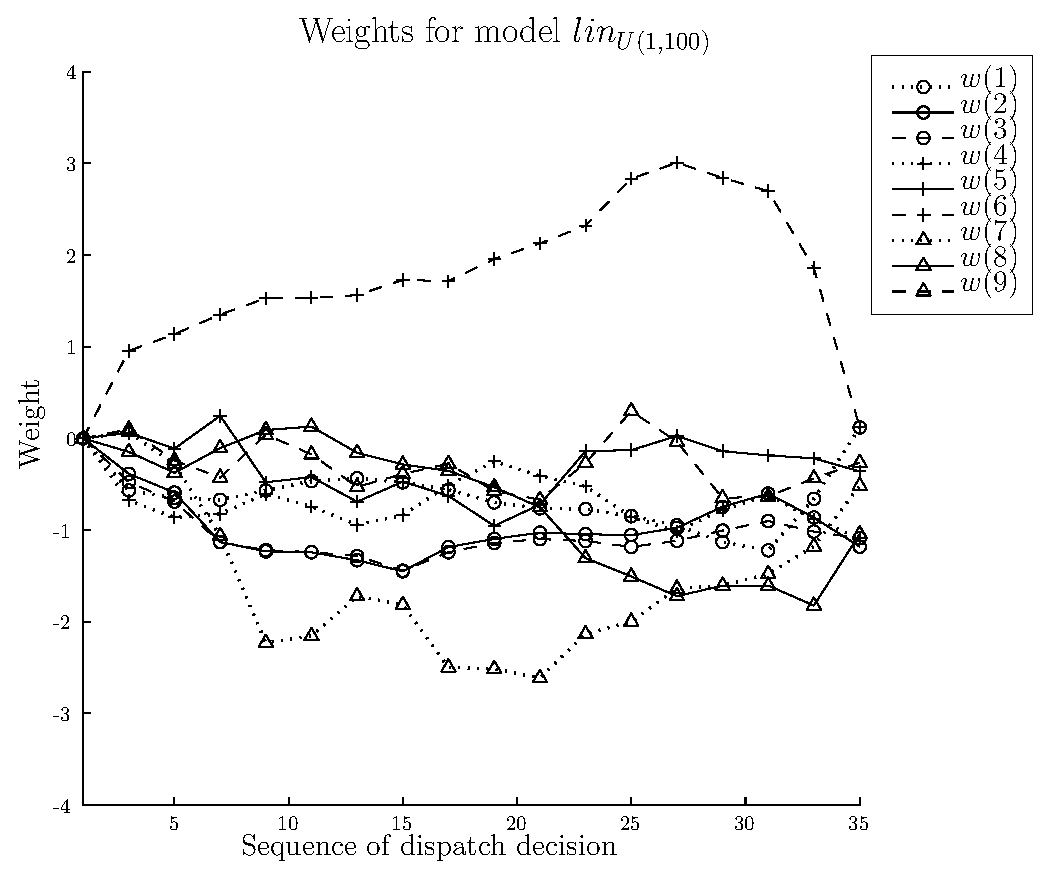
\includegraphics[width=0.85\columnwidth]{figs/fig6_weights0_100.eps}
\includegraphics[width=0.85\columnwidth]{figs/fig6_weights50_100.eps}
\caption{Weights of features as a function of sequence of dispatching decisions, for test data $U(1,100)$ (top) and $U(50,100)$ (bottom).}
\label{fig:variedweights}
\end{figure}


%\begin{figure}[b!]
%\centering
%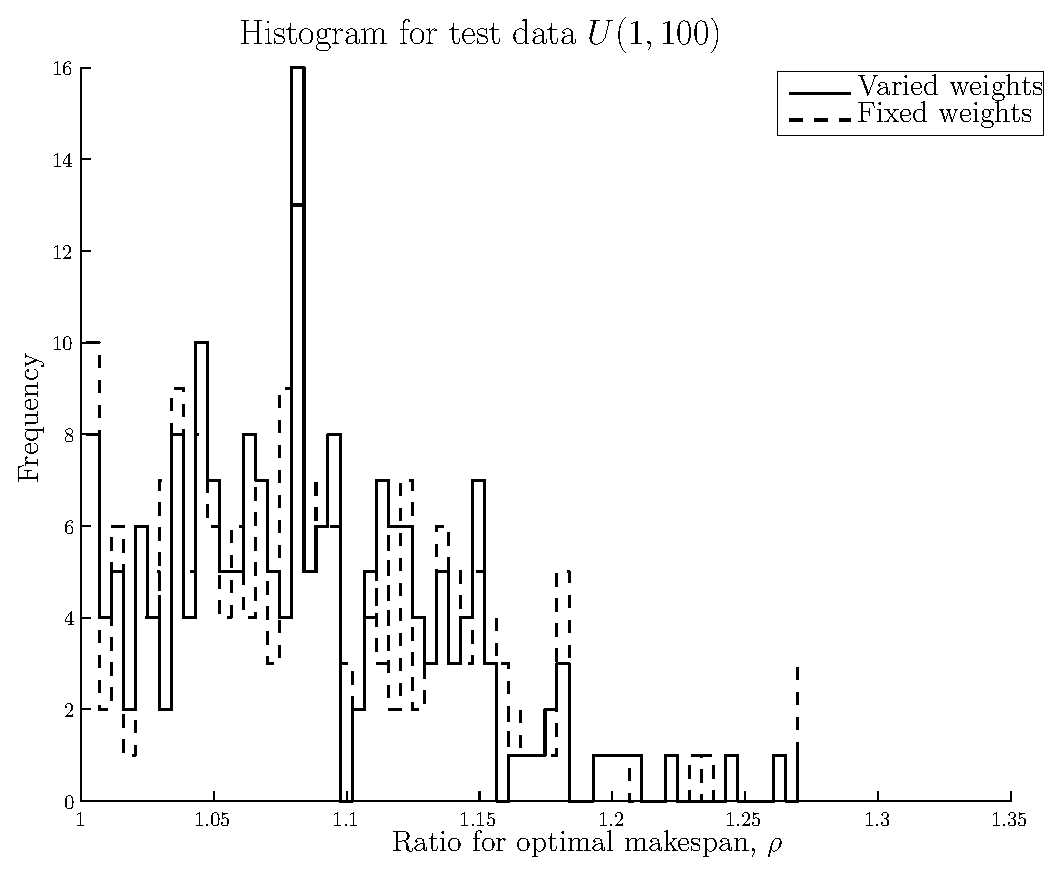
\includegraphics[width=0.49\columnwidth]{figs/fig5_fixed_0_100.eps}
%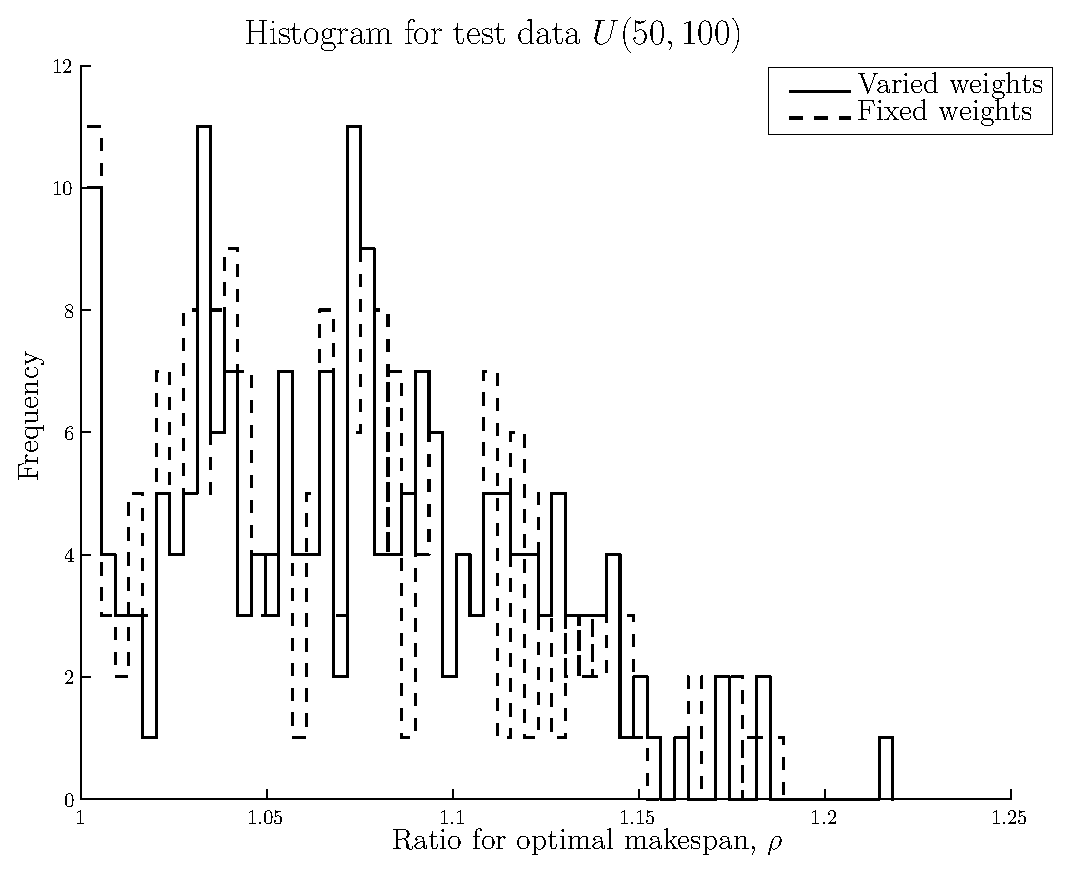
\includegraphics[width=0.49\columnwidth]{figs/fig5_fixed_50_100.eps}
% %\caption{Histogram of ratio from optimum makespan using models $lin_{U(R,100)}$ and $lin_{U(R,100),\textrm{fixed }w}$ for $R=1$ (left) and $R=50$ (right).}
%\label{fig:fixedweights}
%\end{figure}

\begin{table}[h!]
 {\footnotesize
 \begin{center}
  \begin{tabular}{|c|l|l|ccccc|}
   \hline\hline
   & model & test set & mean & std    & med    & min    & max   \\ \hline
\#1 & $lin_{U(1,100)}$ & $U(1,100)$ & 1.0844 & 0.0535 & 1.0786 & 1.0000 & 1.2722  \\
\#2 & $lin_{U(1,100),\textrm{fixed }w}$ & $U(1,100)$ & 1.0862 & 0.0580 & 1.0785 & 1.0000 & 1.2722   \\
\#3 & $lin_{U(50,100)}$ & $U(50,100)$ & 1.0724 & 0.0446&1.0713 & 1.0000 & 1.2159  \\
\#4 & $lin_{U(50,100),\textrm{fixed }w}$ & $U(50,100)$ &  1.0695 & 0.0459 & 1.0658 & 1.0000 & 1.2201  \\
%#1 and #2 are the same distribution
%#3 and #4 are the same distribution
   \hline\hline
  \end{tabular}
 \end{center}}
\caption{Mean value, standard deviation, median value, minimum and maximum values of the ratio from optimum makespan, $\rho$, on models $lin_{U(1,100)}$, $lin_{U(50,100)}$, $lin_{U(1,100),\textrm{fixed }w}$ and $lin_{U(50,100),\textrm{fixed }w}$ for corresponding test sets.}
 \label{tbl:fixedvsvaried}
\end{table}


\begin{table}[h!]
 {\footnotesize
 \begin{center}
  \begin{tabular}{|c|l|l|ccccc|}
   \hline\hline
   & model & test set & mean & std    & med    & min    & max   \\ \hline
\#1 & $lin_{U(1,100),\textrm{fixed }w}$ & $U(1,100)$ & 1.0862 & 0.0580 & 1.0785 & 1.0000 & 1.2722   \\
\#2 & $lin_{U(50,100),\textrm{fixed }w}$ & $U(1,100)$ & 1.0706 & 0.0493 & 1.0597 & 1.0000 & 1.2204  \\
\#3 & $lin_{U(1,100),\textrm{fixed }w}$ & $U(50,100)$ &   1.1356 & 0.0791 & 1.1296 & 1.0000 & 1.5284  \\
\#4 & $lin_{U(50,100),\textrm{fixed }w}$ & $U(50,100)$ &  1.0695 & 0.0459 & 1.0658 & 1.0000 & 1.2201  \\
%#4 and #3 are the same distribution
   \hline\hline
  \end{tabular}
 \end{center}}
 \caption{Mean value, standard deviation, median value, minimum and maximum values of the ratio from optimum makespan, $\rho$, for the test sets $U(1,100)$ and $U(50,100)$, on both fixed weight models $lin_{U(1,100),\textrm{fixed }w}$ and $lin_{U(50,100),\textrm{fixed }w}$.}
 \label{tbl:diffdatadistr:fixed}
\end{table}


\section{Summary and conclusion}
% {\bf Give a brief summary of what was done in this paper and what was achieved, one small paragraph.}
In this paper, a supervised learning linear priority dispatch rules ($lin$) is investi\-gated to find optimal schedules for JSSP w.r.t. minimum makespan. The $lin$-model uses a heuristic strategy such that jobs are dispatched corresponding to the feature set that yielded the highest proportional probability output \eqref{eq:lin}. The linear priority dispatch rules showed clear superiority towards single priority-based dispatch rules. The method of generating training data is  critical for the framework's robustness.  

The framework is not as robust with respect to different data distribution in some cases, and thus cannot be used interchangeably for training and testing and still maintain satisfactory results. Most features were of similar weight between the two data distributions (cf., Table~\ref{tbl:features}), however, there are some slight discrepancies between the two distributions, e.g. $\bar{w}(5)$, which could explain the difference in performance between $lin_{U(1,00)}$ and $lin_{U(50,100)}$.  

There is no statistical difference between using the linear model with varied or fixed weights when using a corresponding test set, so it is sufficient to apply only the mean varied weight, no optimization of the weight parameters is needed. It is noted that some of the robustness between data distribution is lost by using fixed weights. Hence, when dealing with a test set of known data distributions, it is sufficient to use the simpler fixed model $lin_{U(R,100),\textrm{fixed }w}$, however when the data distribution is not known beforehand, it is best to use the slightly more complex varied weights model, and inferring from the experimental data rather use $lin_{U(50,100)}$ to $lin_{U(1,100)}$.

It is possible for a JSSP problem to have more than one optimal solution. However for the purpose of this study, only one optimal solution used for generating training data is sufficient. But clearly the training data set is still corrupted because of multiple ways of representing the same or different (yet equally optimal w.r.t minimum makespan) optimal schedule. One way of overcoming this obstacle is applying mixed integer programming for each possible suboptimal choice, with the current schedule as its initial value to make it absolutely certain that the choice is indeed suboptimal or not. 

% still need to be examined along with the different learning strategies
The proposed approach of discovering learned linear priority dispatching rules introduced in this study, are only compared with three common single priority-based dispatching rules from the literature. Although they provide evidence of improved accuracy, other comparisons of learning approaches, e.g. genetic programming, regression trees and reinforcement learning, need to be looked further into. %This is currently underway.

Another possible direction of future research is to extend the obtained results to different types of scheduling problems, along with relevant features. The efficiency of this problem solver will ultimately depend on the skills of plausible reasoning and how effectively the features extrapolate patterns yielding rules concerning optimal solutions, if they exist.

The main drawback of this approach is in order for the framework to be applicable one needs to know optimal schedules and their corresponding features in order to learn the preference, which may be difficult if not impossible to compute beforehand for some instances of JSSP using exact methods.

\bibliographystyle{splncs}
\bibliography{biblio}

\end{document}

